\documentclass[a4paper,12pt]{article}
\usepackage[utf8]{inputenc}
\usepackage[T1]{fontenc}
\usepackage{amsmath}
\usepackage{graphicx}
\usepackage{geometry}
\geometry{margin=1in}
\usepackage{float}
\usepackage{float}
\usepackage{url}

\title{Solving the Single-Source Unsplittable Flow Problem with Metaheuristic Approaches}
\author{\\Aleksa Toroman 84/2018 \\\\ University in Belgrade, Faculty of Mathematics}
\date{\today}

\begin{document}

\maketitle

\newpage
\renewcommand{\contentsname}{Table of contents}
\tableofcontents

\newpage

\section{Introduction}

The Single-Source Unsplittable Flow Problem (SSUFP) is a well-known problem in network flow optimization. Given a graph $G = (V, E)$ with a source vertex $s$ and a collection of sinks $t_1, \ldots, t_k$ associated with integer demands $\rho_1, \ldots, \rho_k$, the goal is to route a single flow path from the source $s$ to each sink $t_i$ such that the total flow across any edge $e \in E$ does not exceed the edge’s capacity $c(e)$. Formally, the objective is to minimize the maximum ratio $\frac{f(e)}{c(e)}$ over all edges, where $f(e)$ is the total flow routed across edge $e$.

\

\noindent \textbf{Problem Statement:}

\begin{itemize}
    \item \textbf{Instance:} A directed graph $G=(V, E)$ with edge capacities $c: E \to \mathbb{Z}^+$, a source node $s$, and $k$ sinks $t_1, \ldots, t_k$, each with a demand $\rho_i$. Each demand $\rho_i$ must be routed along a single path from $s$ to $t_i$. Additionally, each vertex can have any number of sinks.
    \item \textbf{Objective:} Route each demand in such a way that the total flow routed across any edge $e \in E$ is bounded by its capacity, $c(e)$.
    \item \textbf{Measure:} Minimize the maximum congestion, defined as $\max_{e \in E} \frac{f(e)}{c(e)}$.
\end{itemize}

\noindent The SSUFP is an NP-hard problem, meaning that there is no known polynomial-time algorithm that can solve all instances optimally. The difficulty of the problem lies in the fact that flows cannot be split across multiple paths for each demand; every demand must be routed along a single path. This constraint introduces significant challenges in finding feasible flow paths, especially as the number of demands or the size of the network increases. \\


\noindent \textbf{Complexity and Challenges:}

\noindent Several factors increase the complexity of the problem:

\begin{itemize}
    \item \textbf{Edge Congestion:} Ensuring that no edge exceeds its capacity is challenging when multiple demands compete for the same edges.
    \item \textbf{Path Selection:} Selecting the right paths for each demand is crucial to avoid overloading the network.
    \item \textbf{Scalability:} As the number of demands or the size of the network increases, the number of possible path combinations grows exponentially, making the problem harder to solve.
\end{itemize}

\noindent \textbf{Known Algorithms:}

\

\noindent Despite the complexity, there are approximation algorithms available that provide good solutions in practice. Some notable results include:
\begin{itemize}
    \item A 2-approximation algorithm for minimizing congestion exists when certain conditions are met, meaning that the algorithm can find a solution with at most twice the optimal congestion.
    \item The problem is approximable within a factor of 3.23 for directed graphs, which provides a performance guarantee on how far the solution is from the optimal.
    \item It is also known that no approximation algorithm can achieve a performance better than \( \frac{3}{2} - \epsilon \) for any $\epsilon > 0$, demonstrating the inherent difficulty of the problem.
\end{itemize}

\noindent In addition to these approximation algorithms, here we are covering metaheuristic approaches such as Simulated Annealing, Genetic Algorithms, and Variable Neighborhood Search offer heuristic methods to find near-optimal solutions. These algorithms are particularly useful for large instances where exact methods become impractical.

\

\noindent The remainder of this report will explore metaheuristic approaches to solving the SSUFP, focusing on their implementation and the quality of the solutions they provide.

\section{Research Methodology}

The research for solving the Single-Source Unsplittable Flow Problem (SSUFP) was conducted in several stages, each contributing to the overall understanding and development of a practical solution. The following steps outline the methodology used in this project:

\begin{enumerate}
    \item Getting familiar with the problem and reading existing literature.
    \item Creating a custom graph textual representation.
    \item Developing a graph generation library for instance creation.
    \item Building core infrastructure classes in Python, including representations for the graph, demands, and utilities.
    \item Implementing algorithms, including Brute Force, Simulated Annealing, and Genetic Algorithm.
    \item Analyzing and evaluating the results of the implementations.
\end{enumerate}

\subsection{Getting Familiar with the Problem and Literature Review}

The first phase of the project was dedicated to understanding the Single-Source Unsplittable Flow Problem (SSUFP). I began by exploring its mathematical formulation and related optimization challenges. To build a solid foundation, I reviewed relevant literature and research on unsplittable flow and NP-hard network problems, which helped me grasp the complexities and common solution approaches.

\section{Graph Representation and Infrastructure}

\subsection{Creating a Custom Graph Textual Representation}

To represent the input graph for the Single-Source Unsplittable Flow Problem, a custom textual format was designed. This format is easy to parse and process programmatically, and it captures all necessary details, including vertices, edges, capacities, and demands for each sink.

\noindent The structure of the graph representation is as follows:

\begin{itemize}
    \item The first line contains the number of vertices.
    \item The second line indicates the number of edges.
    \item The third line identifies the source vertex.
    \item The next \(N\) lines represent each edge in the format: \textit{source vertex, destination vertex, capacity}, where the graph is directed.
    \item After the edges, there is a line containing the number of sink vertices.
    \item The remaining lines correspond to the sink vertices, where each line contains the index of the vertex, the number of sinks that vertex has, and their respective demands.
\end{itemize}

\noindent \textbf{Example Representation:}

\begin{verbatim}
5
7
1
1 2 7
1 3 3
2 4 6
2 3 5
2 5 4
5 4 2
1 5 5
2
4 1 3
3 2 2 1
\end{verbatim}

\noindent In this example:
\begin{itemize}
    \item The graph has 5 vertices and 7 edges.
    \item Vertex 1 is the source.
    \item The edges are represented as directed connections between vertices, with specified capacities.
    \item There are 2 sink vertices, with vertex 3 having two demands (2 and 1), and vertex 4 having one demand (3).
\end{itemize}

\begin{figure}[H]
\centering
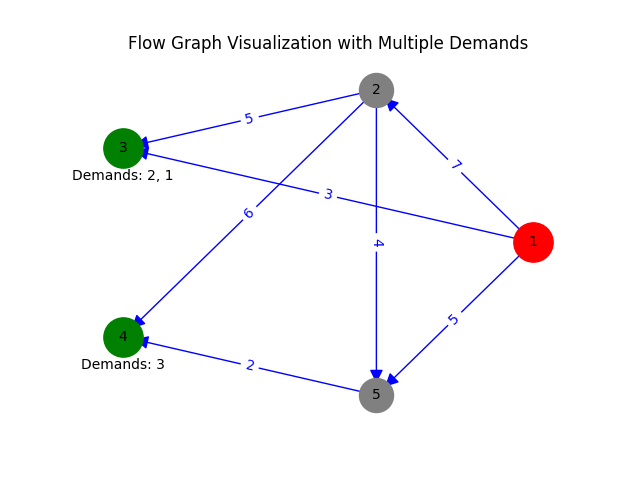
\includegraphics[width=100mm]{graph-1.png}
\caption{Example graph problem instance}
\label{fig:graph_example}
\end{figure}

\noindent \textbf{Example Solution:}
\begin{verbatim}
Path for Flow (Source: 1, Sink: 4, Flow: 3): [1, 2, 4]
Path for Flow (Source: 1, Sink: 3, Flow: 2): [1, 3]
Path for Flow (Source: 1, Sink: 3, Flow: 1): [1, 2, 3]
All constraints satisfied.
Maximum Flow-to-Capacity Ratio: 0.67
\end{verbatim}

\subsection{Graph Generation Library for Instance Creation}

In order to effectively test the algorithms, a graph generation library was developed due to the lack of a pre-existing dataset for the Single-Source Unsplittable Flow Problem (SSUFP). Initially, I created a few simple examples that could be manually calculated, serving as a basic test for the algorithms. However, for larger-scale testing and analysis, i implemented a mechanism to generate random graph instances of various sizes. One challenge was ensuring the generated graphs consistently provided valid paths between the source and sink vertices, which required several iterations to refine the generator.

\

\noindent The graph generation uses the NetworkX library in python to create directed random graphs, with adjustments made to tailor the graphs specifically for the SSUFP problem. The process involves the following key steps:

\begin{itemize}
    \item Initial Graph Generation: A random directed graph is generated using the Erdős-Rényi model, with an edge probability that varies depending on the graph size. For small graphs, the edge probability is 0.2, for medium graphs it is 0.15, and for large graphs it is 0.1. These probabilities influence the density of edges in the generated graph.
    
    \item Graph Adjustments: After generating the random graph, certain adjustments are made:
    \begin{itemize}
        \item Outgoing edges from non-source vertices to the source are removed to avoid reverse flow.
        \item Outgoing edges from sink vertices are removed to ensure sinks do not act as intermediate vertices for other flows.
        \item If no path exists between the source and any sink, random "hops" are added between intermediate nodes to create a valid path, ensuring at least one solution exists for each instance.
    \end{itemize}
    
    \item Edge Capacities: Capacities for the edges are assigned randomly within a range of 10 to 40. These capacities represent the maximum flow that each edge can carry.
    
    \item Demand Generation: Demands for sink vertices are generated based on the type of graph. For balanced graphs, each sink vertex typically has 1 or 2 demands, while for large-demand graphs, each sink can have up to 3 demands. The demand values are random integers, but they are kept small compared to the edge capacities to ensure feasible solutions. Also, each demand cannot be higher than the capacity of any edge in defined graph.
    
    \item Graph Sizes:
    \begin{itemize}
        \item Small Graphs: Small instances contain between 5 and 10 nodes, with 1 to 3 demands.
        \item Medium Graphs: Medium instances range from 15 to 25 nodes, with 3 to 6 demands.
        \item Large Graphs: Large instances contain between 30 and 50 nodes, with 5 to 10 demands.
    \end{itemize}
    
    \item Graph Serialization: After generating and adjusting the graph, it is serialized into a given text format described earlier. The serialization includes all nodes, edges, capacities, and demands. The generated graph is saved as a text file, where each graph's filename includes a hash for uniqueness.
    
\end{itemize}

\subsection{Building Core Infrastructure Classes in Python}

To effectively implement and test various algorithms for solving the Single-Source Unsplittable Flow Problem (SSUFP), several core infrastructure components were developed in Python. These include essential classes to represent the graph, demands, and results, as well as utility functions used by the algorithms. The code was designed to be modular and reusable, supporting various hyperparameter configurations and testing scenarios.

\

\noindent \textbf{Core Classes:}

\begin{itemize}
    \item \textbf{Graph Class}: This class represents the underlying network with nodes and edges, storing relevant information such as capacities and connections between vertices as well as list of demands.
    \item \textbf{Demand Class}: Each demand corresponds to a specific sink vertex and its associated demand value, ensuring that the each demand in graph must be routed unsplittably along a single path.
    \item \textbf{Result Class}: This class holds the results of each algorithm run, tracking information such as the time taken, whether the solution was feasible, and the objective function value.
    \item \textbf{Statistics Class}: For each algorithm run, a separate 'reports.csv' file is generated, containing detailed information about the results. This data is later aggregated to compare the performance of different algorithms and parameter configurations.

\end{itemize}

\noindent \textbf{Utility Functions:}
In addition to the core classes, several utility functions were implemented to assist the algorithms:
\begin{itemize}
    \item \textbf{Feasibility Check}: A utility function checks whether a solution is feasible by verifying that the flow on each edge does not exceed its capacity. This operation is of polynomial time complexity.
    \item \textbf{Random Path Finder}: A depth-first search (DFS) based function is used to find random paths between two nodes.
\end{itemize}

\noindent \textbf{Hyperparameter Support:}
The infrastructure is flexible enough to allow passing different hyperparameters to various algorithms. Similar to the grid search in libraries like \textit{scikit-learn}, different combinations of hyperparameters can be tested to optimize the performance of the algorithms. Parameters such as cooling rate for Simulated Annealing or population size for the Genetic Algorithm can be modified this way.

\

\noindent \textbf{Automation and Result Logging:}
A root file structure was designed to automatically run different algorithms and store the results in a well-organized format. The results for each algorithm run are saved in CSV files, which include details such as:
\begin{itemize}
    \item Algorithm used
    \item Hyperparameters used
    \item Time taken by the algorithm
    \item Whether the solution was feasible
    \item Objective function value (optimization target)
    \item ...
\end{itemize}

\noindent This mechasnism also allows to store different artifacts such as different kinds of plots in well organized structure during the algorithm execution.

\

\noindent Additionally, a command-line interface allows users to specify which algorithms to run, and where is the root folder of given example instances. The results are automatically exported into an csv file in above mentioned file structure, making it easier to analyze and compare the performance of different algorithms across multiple instances.

\

\noindent Below is an example of the folder structure and a snippet from the result log:

\begin{figure}[H]
    \centering
    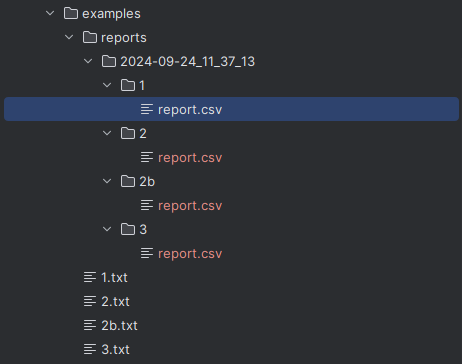
\includegraphics[width=0.5\textwidth]{reports-structure.png}
    \caption{Screenshot of result file structure and log}
\end{figure}

\begin{figure}[H]
    \centering
    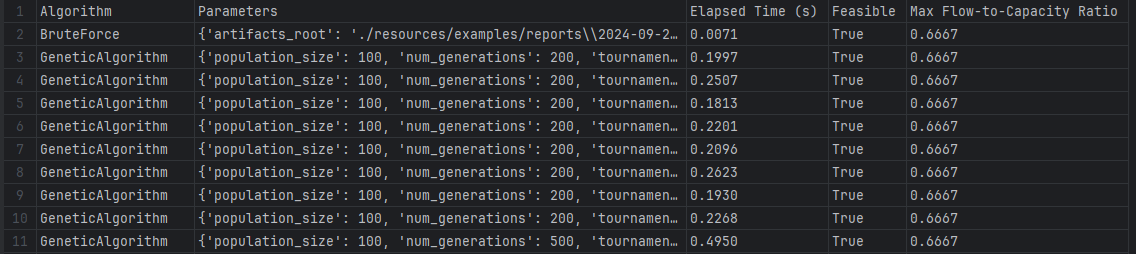
\includegraphics[width=0.5\textwidth]{report-snippet.png}
    \caption{Snippet of result log showing algorithm details and performance}
\end{figure}

\section{Algorithm Overview}

\subsection{Used Algorithms}

To solve the Single-Source Unsplittable Flow Problem (SSUFP), several algorithms were implemented, each offering different approaches to finding feasible and near-optimal solutions. The algorithms developed include both exact and metaheuristic techniques:

\begin{itemize}
    \item \textbf{Brute Force}: A straightforward approach that explores all possible paths from the source to each sink and evaluates all combinations of paths to find the best feasible solution. Due to the problem's NP-hard nature, this method is only feasible for small instances.
    
    \item \textbf{Simulated Annealing}: A metaheuristic algorithm inspired by the annealing process in metallurgy. It starts with an initial solution and explores neighboring solutions, gradually reducing the likelihood of accepting worse solutions as the temperature decreases. This allows for exploration of the solution space while avoiding getting stuck in local optima.
    
    \item \textbf{Variable Neighborhood Search (VNS)}: This algorithm systematically changes the neighborhood structures during the search. By altering the neighborhood, VNS explores different parts of the solution space, switching between local searches to escape local optima and find better solutions.
    
    \item \textbf{Genetic Algorithm (GA)}: A population-based optimization algorithm that mimics natural selection. The algorithm generates an initial population of solutions and evolves them using operations like crossover and mutation. Over several generations, the population converges towards a feasible and near-optimal solution.
\end{itemize}

\noindent Each of these algorithms were implemented in Python, leveraging the core infrastructure classes and utility functions described earlier.

\subsection{Brute Force Algorithm}

The Brute Force method retrieves all possible paths from the source to each sink, including multiple demands for the same sink. Using the NetworkX library to find simple paths, this works well for small graphs.

\noindent The algorithm then generates all route combinations using the Cartesian product of the paths and checks each for feasibility. For feasible solutions, it calculates the maximum congestion.

\noindent While effective for small graphs, this approach becomes impractical for larger graphs due to the exponential growth in path combinations.

\

\noindent \textbf{Example:}
In one example graph with 11 vertices and 3 sink nodes, where two of the sink nodes have two demands each, the number of possible paths for each demand is as follows:

\begin{verbatim}
Number of paths for each demand: [19, 19, 38, 38, 11]
\end{verbatim}

\noindent This results in a total of 5,734,124 combinations. Out of these, only 3,041 combinations were feasible. The Brute Force algorithm completed in 63.03 seconds for this instance.

\begin{figure}[H]
    \centering
    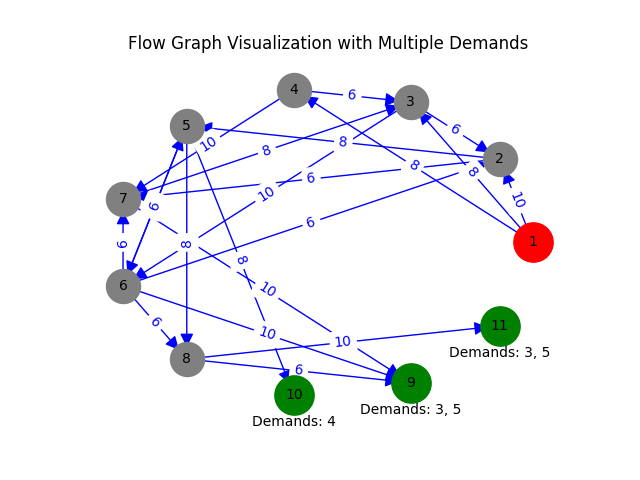
\includegraphics[width=0.5\textwidth]{brute-force-example.png}
    \caption{Example graph solved using brute force algorithm}
\end{figure}

\begin{itemize}
    \item Total combinations: 5,734,124
    \item Feasible combinations: 3,041
    \item Time taken: 63.03 seconds
\end{itemize}

\noindent  While Brute Force provides an exact solution, its time complexity grows exponentially, making it impractical for graphs with many paths and multiple demands. This highlights the need for more scalable, approximate methods like Simulated Annealing, VNS and Genetic Algorithms for larger instances.

\subsection{Common Stoppage Criteria for Heuristic Algorithms}

All heuristic algorithms in this project are controlled by two main criteria: maximum execution time and the no\_improvement\_threshold. These criteria ensure that algorithms stop either after a set time or when no further improvements are made.

\begin{itemize}
    \item \textbf{Maximum Time}: Each algorithm runs for a set time limit, ranging from 20 seconds for small graphs to 80 seconds for larger ones, to balance runtime and exploration.
    \item \textbf{No\_Improvement\_Threshold}: This defines how many iterations can occur without improvement. For Simulated Annealing, this threshold is higher (150-250 iterations), while for Genetic Algorithms, it’s lower (100-150 iterations).
\end{itemize}

\noindent These limits can be adjusted for more exploration if computational resources allow but are kept within reasonable bounds to ensure efficient testing and meaningful results.


\subsection{Generating Neighbor Solution}

In Simulated Annealing, Variable Neighborhood Search (VNS), and Genetic Algorithms, generating a neighbor solution is key to exploring new options. This function goal is to make randomized slight adjustments in current solution and can be implement in various ways based on problem and solution representation. In our case, this function works in following way:

\begin{itemize}
    \item It randomly selects demand in available list of demands.
    \item It randomly selects two nodes in the previously selected demand flow path (including the source and sink).
    \item A new path between these two nodes is generated using randomized depth-first search (DFS).
    \item The new path replaces the selected portion of the original flow path.
\end{itemize}

To optimize this process:
\begin{itemize}
    \item Cycles are avoided by excluding nodes that would form a loop.
    \item The current path is excluded from consideration to ensure a true modification.
\end{itemize}

\noindent This method is used in Simulated Annealing for exploring new solutions, in VNS in both shaking and local search step, and in Genetic Algorithms during mutation to introduce variety.

\subsection{Goal Function}

In this problem, there are two key objectives:
\begin{itemize}
    \item Find a feasible solution where the flow on every edge does not exceed its capacity.
    \item Minimize the congestion, measured by: 
    \[
    \max_{e \in E} \frac{f(e)}{c(e)},
    \]
    where \( f(e) \) is the total flow on edge \( e \) and \( c(e) \) is its capacity.
\end{itemize}

To achieve this, the goal function follows these rules:
\begin{itemize}
    \item Feasible solutions are always prioritized over non-feasible ones.
    \item Among feasible solutions, the one with the lowest max\_flow\_to\_capacity ratio is considered the best.
    \item Non-feasible solutions are compared based on the total overflow across all edges, with smaller total overflow being better. This helps guide the algorithm toward feasible solutions.
\end{itemize}

\

\noindent \textbf{Goal Function Pseudocode:}

\begin{verbatim}
function calculate_score():
    total_penalty = 0
    feasible = True
    
    edge_flows = calculate_edge_flows()
    capacities = edges

    for each edge in edge_flows:
        flow = edge_flows[edge]
        capacity = capacities[edge]

        if flow > capacity:
            overflow = flow - capacity
            total_penalty += overflow
            feasible = False

    if feasible:
        max_flow_to_capacity_ratio = calculate_max_flow_to_capacity_ratio()
        return 1 - max_flow_to_capacity_ratio
    else:
        return -(1 + total_penalty)
\end{verbatim}

This function ensures that feasible solutions with lower congestion are favored, while non-feasible solutions are penalized based on how much they overflow. This strategy helps navigate the search space toward finding feasible, optimal solutions.

\subsection{Simulated Annealing}

The Simulated Annealing algorithm was implemented to explore the solution space for the Single-Source Unsplittable Flow Problem (SSUFP). The goal is to find feasible solutions while minimizing the congestion, using the previously defined goal function.

\

\noindent \textbf{Parameter Grid:}

\begin{verbatim}
sa_param_grid = {
    'initial_temp': [3000, 5000],
    'cooling_rate': [0.99, 0.95]
}
\end{verbatim}

\noindent \textbf{Algorithm Overview:}
\begin{itemize}
    \item The algorithm starts with an initial solution where, for each demand, a random path is generated from the source to the sink. If a sink has multiple demands, the method is called separately for each.
    \item At each iteration, a neighbor solution is generated by altering the current flow paths as described earlier.
    \item The goal function is used to evaluate each solution, and a solution is accepted based on its score. If the new solution is worse, an acceptance probability is calculated based on the current temperature, allowing worse solutions to be accepted with some likelihood to avoid local optima.
    
    \item The temperature gradually decreases according to the cooling rate, reducing the likelihood of accepting worse solutions as the algorithm progresses.
\end{itemize}

\noindent This standard approach to Simulated Annealing leverages the flexibility of the neighbor generation function and the goal function to guide the search toward feasible and optimal solutions.

\subsection{Variable Neighborhood Search (VNS)}

Variable Neighborhood Search (VNS) is a metaheuristic algorithm that systematically explores different neighborhoods of the solution space. In this implementation, neighborhoods are defined based on the number of demands whose paths will be modified during the shaking process. The algorithm also alternates between small, incremental changes and more significant rerouting of paths.

\

\noindent \textbf{Parameter Grid:}

\begin{verbatim}
vns_param_grid = {
    'k_min': [0, 1, 2],
    'k_max': [3, 5],
    'move_prob': [0.1, 0.2],
    'reroute_entire_path_prob': [0.3, 0.5]
}
\end{verbatim}

\noindent \textbf{Shaking Process:}
\begin{itemize}
    \item Each neighborhood defines how many demands to modify. The number of demands increases as the search moves through larger neighborhoods.
    \item For each demand selected in the shaking process, there is a probability (between 0.3 and 0.5 based on given params configuration) of performing a full rerouting from the source to the sink, which replaces the entire path with a new one. Otherwise, a small modification is made to the path using the neighbor generation method.
\end{itemize}

\noindent This dual approach allows the algorithm to explore both small and large modifications, balancing local exploration with more significant changes when necessary.

\

\noindent \textbf{Local Search:}
After shaking, the local search is applied to refine the solution. The goal is to iteratively improve the solution by making small changes to individual demands. The process works as follows:

\begin{itemize}
    \item A copy of the current solution is made.
    \item A randomized order of demands is generated to explore possible improvements.
    \item For each demand, a neighboring solution is generated by modifying the flow path for that demand.
    \item The score of the modified solution is calculated using the goal function. If the new score is better, the current solution is replaced with the modified one, and the search continues.
    \item This process repeats until no further improvements can be made, ensuring the local optimum is reached.
\end{itemize}

\noindent This combination of shaking and local search allows VNS to efficiently escape local optima by dynamically adjusting the neighborhood size and exploring a variety of solution modifications.

\subsection{Genetic Algorithm (GA)}

The Genetic Algorithm (GA) was implemented to solve the Single-Source Unsplittable Flow Problem (SSUFP) by mimicking the process of natural selection. This involves creating an initial population, selecting the best solutions, and applying crossover and mutation to evolve new generations.

\

\noindent \textbf{Parameter Grid:}

\begin{verbatim}
ga_param_grid = {
    'population_size': [100, 200, 400],
    'num_generations': [300, 500],
    'tournament_size': [5, 10],
    'elitism_size': [10, 20],
    'mutation_prob': [0.05, 0.1, 0.15, 0.2]
}
\end{verbatim}

\textbf{Algorithm Overview:}

\begin{itemize}
    \item \textbf{Initial Population:} The initial population is generated in the same way as the initial solution for Simulated Annealing, by finding random paths for each demand. This process is repeated based on the size of the population.
    
    \item \textbf{Selection:} Tournament-based selection is used to choose parents for crossover. In each tournament, a subset of individuals is selected at random, and the one with the best fitness is chosen as a parent.
    
    \item \textbf{Crossover:} Uniform crossover is applied to combine two parents and create two children. For each demand, there is a 50\% chance of taking the demand path from one parent or the other. The unselected demand path goes to the other child, ensuring both children are formed by mixing parts of their parents' paths. This process repeats for all demands.

    \item \textbf{Mutation:} Each demand path in the child solution is mutated with a given probability (mutation\_prob). The mutation is performed using the previously described \textit{generate\_neighbor} method, which modifies part of the path.
\end{itemize}

\begin{verbatim}
function mutate(mutation_prob):
    for each demand path in solution:
        if random() < mutation_prob:
            mutate the demand path using generate_neighbor
\end{verbatim}

\noindent The fitness of each solution is determined by the goal function described earlier. After several generations, the best solutions evolve toward feasible and optimal paths, balancing exploration and exploitation through crossover and mutation.


\section{Results Comparison and Conclusion}\

\begin{figure}[H]
    \centering
    \begin{minipage}{0.32\textwidth}
        \centering
        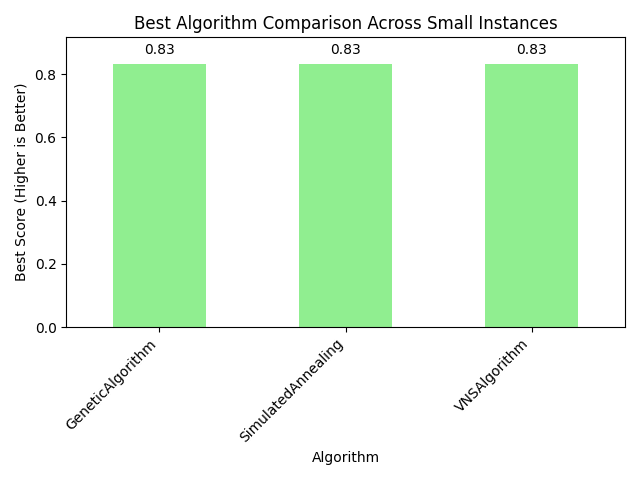
\includegraphics[width=\linewidth]{small_results.png}
        \caption{Best Algorithm Comparison Across Small Instances}
        \label{fig:small_results}
    \end{minipage}\hfill
    \begin{minipage}{0.32\textwidth}
        \centering
        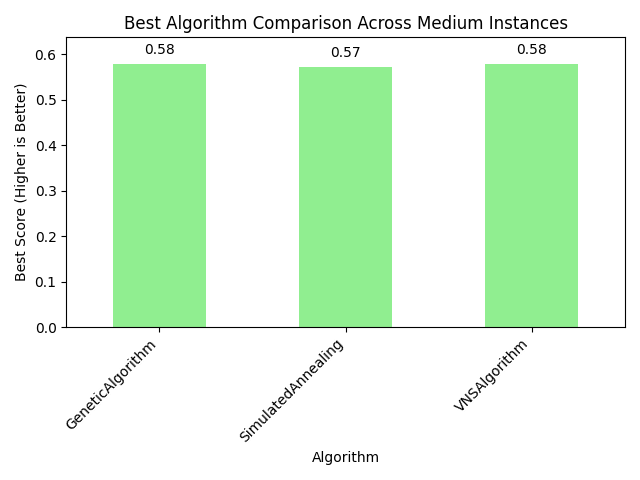
\includegraphics[width=\linewidth]{medium_results.png}
        \caption{Best Algorithm Comparison Across Medium Instances}
        \label{fig:medium_results}
    \end{minipage}\hfill
    \begin{minipage}{0.32\textwidth}
        \centering
        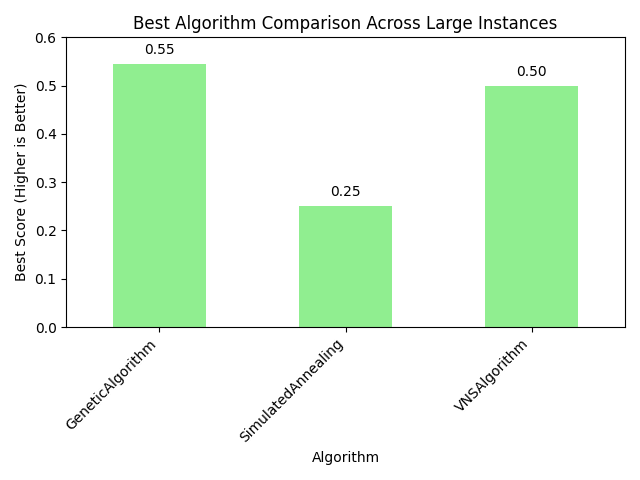
\includegraphics[width=\linewidth]{large_results.png}
        \caption{Best Algorithm Comparison Across Large Instances}
        \label{fig:large_results}
    \end{minipage}
\end{figure}

\subsection{Small Instances}
All three algorithms (Genetic Algorithm, Simulated Annealing, and VNS) perform similarly for small instances, each achieving a best score of 0.83. This suggests that for smaller problem instances, any of the heuristic methods can yield optimal or near-optimal solutions with high reliability.

\subsection{Medium Instances}
The performance remains close among the algorithms for medium instances, with the Genetic Algorithm and VNS slightly outperforming Simulated Annealing. The best scores are around 0.58, indicating that even for medium-sized instances, the algorithms provide comparable results, with a slight advantage for the Genetic Algorithm and VNS.

\subsection{Large Instances}
For large instances, a clearer differentiation is observed. The Genetic Algorithm achieves the highest score at 0.55, followed by VNS at 0.50, while Simulated Annealing lags behind with a score of 0.25. This suggests that for larger, more complex graphs, the Genetic Algorithm and VNS are more effective compared to Simulated Annealing.

\section{Future Improvements}

In the future, I plan to focus more on large-scale graph instances, as small and medium graphs tend to yield similar performances across the algorithms. Expanding the dataset with larger, more complex graphs would provide better insights into the scalability of the solutions. Additionally, I aim to explore other heuristic algorithms, such as Ant Colony Optimization, to compare their effectiveness. For the existing Genetic Algorithm, experimenting with different strategies for crossover and mutation could further improve performance. Finally, optimization techniques and parallelism could be implemented to enhance the runtime efficiency of the program, allowing it to handle larger graphs more quickly.


\clearpage

\section*{References}

\begin{itemize}
    \item Yefim Dinitz, Naveen Garg, and Michel X. Goemans, \textit{On the Single-Source Unsplittable Flow Problem}, SIAM Journal on Computing, Vol. 31, No. 1, pp. 219-235, 2001.
    \item GitHub Repository for Course Materials: \textit{MATF-RI/Materijali-sa-vezbi} \newline
    \url{https://github.com/MATF-RI/Materijali-sa-vezbi}
    \item Problem Definition, \textit{Introduction to the Unsplittable Flow} \newline
    \url{https://www.csc.kth.se/~viggo/wwwcompendium/node125.html}.
\end{itemize}



% Placeholder for results analysis
\end{document}


\end{document}
